\subsection{Administracija sistema}

Administracija sistema odnosi se na dodavanje novih zaposlenih u Nacionalnoj slu\v zbi u sistem, odnosno pravljenje novih naloga, kako bi mogli da mu pristupaju. Tako\dj e, podrazumeva brisanje korisnika iz sistema koji vi\v se ne rade u slu\v zbi. Jo\v s jedan postupak koji se uklju\v cuje u ovaj slu\v caj upotrebe, a mo\v zda i najva\v zniji, je pravljenje backup-a baze podataka.

\begin{figure}[H]
	\centering
	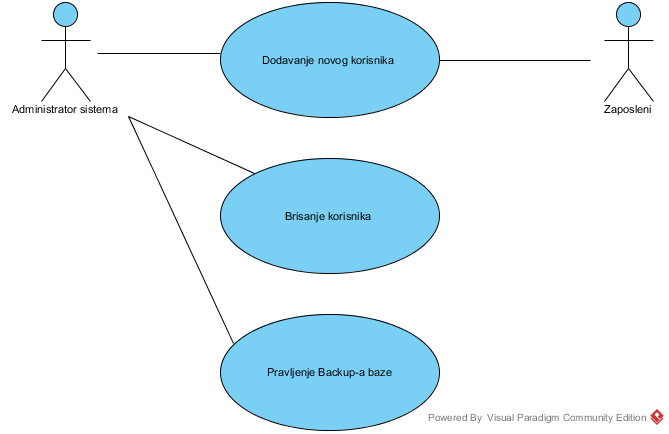
\includegraphics[width=0.8\textwidth]{dijagrami/dijagrami-slucajeva-upotrebe/administracija-sistema.png}
	\caption{Dijagram slu\v cajeva upotrebe procesa "Administracija sistema"}
	\label{dsu: administracija sistema}
\end{figure}

\subsubsection{Slu\v caj upotrebe: Dodavanje novog korisnika}

\label{su: dodavanje novog korisnika}

\noindent U\v cesnici: Administrator sistema (AS), Zaposleni (Z)
\\
\\ Preduslovi: Z je zaposlen u Nacionalnoj slu\v zbi za zapo\v sljavanje. AS ima privilegovan pristup sistemu i ulogova je u sistem.
\\
\\ Postuslovi: AS je uspe\v sno uneo novog korisnika u sistem i Z ima mogu\' cnost logovanja na sistem i pristup podacima.
\\
\\ Glavni tok:
\begin{enumerate}
	\item Z dolazi kod AS u kancelariju i zahteva otvaranje naloga.
	\item AS bira opciju za kreiranje novog naloga.
	\item AS tra\v zi od Z da mu preda li\v cnu kartu.
	\item Z predaje li\v cnu kartu.
	\item AS proverava da li Z ve\' c ima nalog, na osnovu JMBG-a i broja li\v cne karte.
	\begin{itemize}
		\item Ukoliko Z ve\' c ima nalog, AS odustaje od pravljenja novog naloga i slu\v caj upotrebe se ovde zavr\v sava.
		\item Ina\v ce, izvr\v savanje se nastavlja u u koraku 6.
	\end{itemize}
	\item AS popunjava formular.
	\item AS zahteva od Z da uneste \v sifru za nalog.
	\item Z unosi \v sifru u formular.
	\item AS provera sve unete podatke i vr\v si ispravke u slu\v caju unosa pogre\v snog podatka.
	\item AS potvr\dj uje unos.
	\item AS \v stampa potvrdu o uspe\v sno napravljenom nalogu.
	\item AS vra\' ca li\v cnu kartu i predaje potvrdu o nalogu. 
	
\end{enumerate}

\noindent Alternativni tok:
\begin{description}
	\item[A1. Pad sistema] ~\\
	Ukoliko se u bilo kom koraku Glavnog toka dogodi pad sistema na kojem radi AS, AS ponovo pokre\'ce sistem i prijavljuje se na njega.
	\begin{enumerate}
		\item AS proverava da li je formular sa\v cuvan.
		\item Ukoliko jeste, prelazi se na korak 8 Glavnog toka.
		\item Ina\v ce, prelazi se na korak 6 Glavnog toka.
	\end{enumerate}
	\item[A2. Neuspe\v san unos] ~\\
	Ukoliko u koraku 9 Glavnog toka sistem prijavi gre\v sku pri \v cuvanju informacija, AS poku\v sava ponovo. Izvr\v savanje se nastavlja u koraku 5 Glavnog toka.
\end{description}


\subsubsection{Slu\v caj upotrebe: Brisanje korisnika}

\label{su: brisanje korisnika}

\noindent U\v cesnici: Administrator sistema (AS)
\\
\\ Preduslovi: AS ima privilegovan pristup sistemu i ulogova je u sistem. AS je primio zahtev za brisanje korisnika.
\\
\\ Postuslovi: Korisnik je uspe\v sno obrisan iz sistema ili je stanje sistema nepromenjeno.
\\
\\ Glavni tok:
\begin{enumerate}
	\item AS otvara zahtev za brisanje korisnika.
	\item AS pronalazi korinsika u sistemu.
	\item AS bira opciju "Obri\v si korisnika".
	\item Sistem zahteva od AS da potvrdi akciju koju \v zeli da izvr\v si.
	\begin{itemize}
		\item Ukoliko AS pritisne "Da", sistem vr\v si operaciju brisanja.
		\item U suprotnom, nikakve promene nisu na\v cinjene.
	\end{itemize}
\end{enumerate}

\noindent Alternativni tok: /

\subsubsection{Slu\v caj upotrebe: Back-up baze podataka}


\label{su: backup}
\noindent U\v cesnici: Administrator sistema (AS)
\\
\\ Preduslovi: Sistem ispravno funkcioni\v se. AS je ulogovan na sistem i ima privilegovan pristup.
\\
\\ Postuslovi: Backup je uspe\v sno napravljen.
\\
\\ Glavni tok:
\begin{enumerate}
	\item AS proverava da li se trenutno vr\v si neka bitna obrada nad bazom.
	\begin{itemize}
		\item Ukoliko je to slu\v caj, AS \v ceka da se zavr\v si.
		\item U suprotnom, izvr\v savanje se nastavlja u koraku 2.
	\end{itemize}
	\item AS bira da li pravi standardni backup baze ili \v zeli da postavi detaljnije parametre.
	\begin{itemize}
		\item Ukoliko je odabran backup sa parametrima, AS ih pode\v sava.
		\item U suprotnom se prelazi na slede\' ci korak.
	\end{itemize}
	\item AS pokre\' ce pravljenej backup-a.
	\item AS snima backup na memorijski medijum i bele\v zi vreme kada je napravljen.
\end{enumerate}

\noindent Alternatinvni tok: /

\subsubsection{Dijagrami sekvence}

\begin{figure}[H]
	\centering
	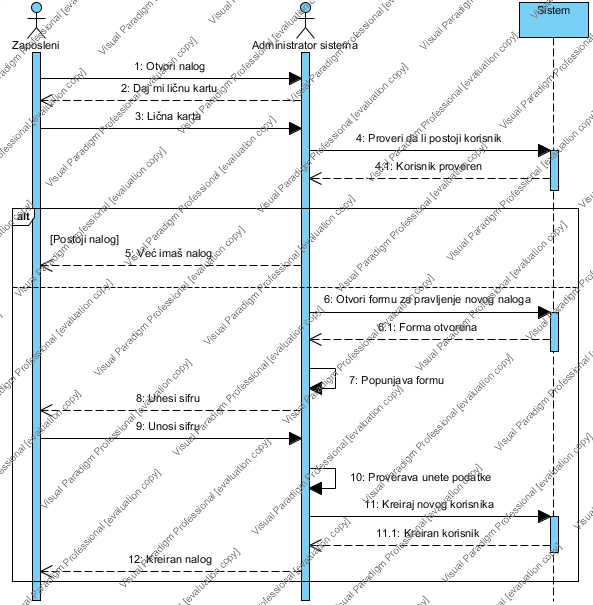
\includegraphics[width=0.6\paperwidth]{dijagrami/dijagrami-sekvence/dodavanje-novog-korisnika.png}
	\caption{Dijagram sekvence slu\v caja upotrebe ''Dodavanje novog korisnika'' (\ref{su: dodavanje novog korisnika}).}
\end{figure}

\newpage

\begin{figure}[H]
	\centering
	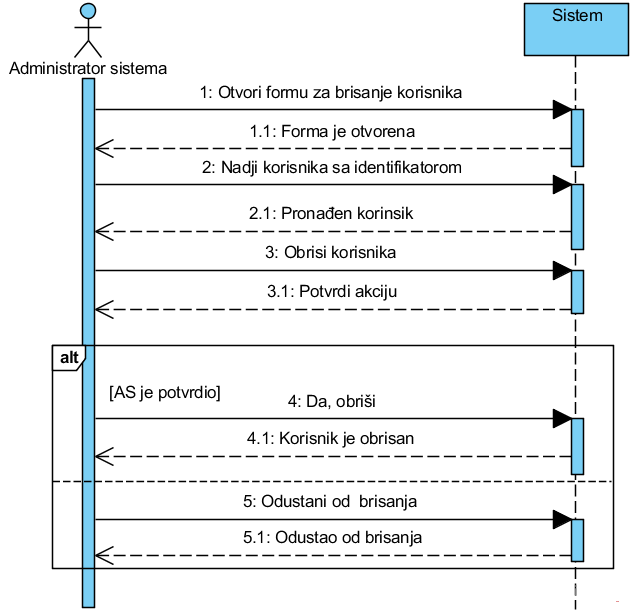
\includegraphics[width=0.7\paperwidth]{dijagrami/dijagrami-sekvence/brisanje-korisnika.png}
	\caption{Dijagram sekvence slu\v caja upotrebe ''Brisanje korisnika' (\ref{su: brisanje korisnika}).}
\end{figure}

\newpage

\begin{figure}[H]
	\centering
	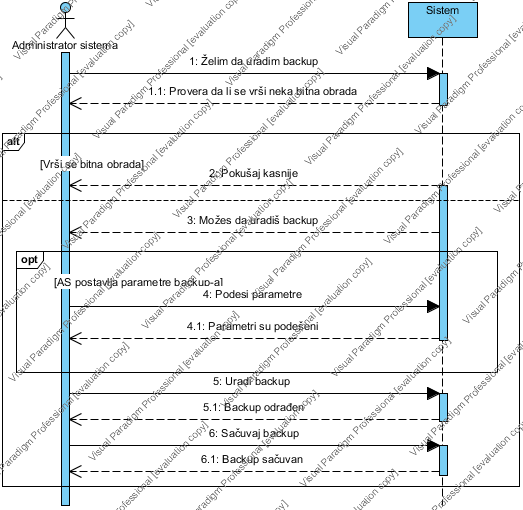
\includegraphics[width=0.95\textwidth]{dijagrami/dijagrami-sekvence/backup.png}
	\caption{Dijagram sekvence slu\v caja upotrebe ''Back-up baze podataka'' (\ref{su: backup}).}
\end{figure}